% formato-detallado.tex
% Esqueleto para escribir tesis en la FCFM.
% Actualización del original fcfmskel.tex
% --- ATENCIÓN--
% Hay varias instrucciones comentadas. Es necesario quitar el
% comentario a alguna de ellas y comentar la instrucción de arriba.
% Se marcan con %----

\documentclass[fisica]{fcfmtesis}      %----tesis de fisica
% Opciones     ^^^^^^  posibles son:
% fisica (Lic. Física), fisapl (Lic. Física Aplicada)
% pfa1 (M.C. Ciencias, Física Aplicada), pfa2 (D.C. Ciencias, Física Aplicada)
% matematicas (Lic. Matemáticas), lma (Lic. Mat. Aplicadas), actuaria (Lic. Actuaría)
% mem (Maestría en Educacuón Matemática)
%\include{parche}  %----para tener tres vocales, define \vocalc


\usepackage[T1]{fontenc}		   %%% fonts y unicode UTF8
\usepackage[utf8]{inputenc}        
% \usepackage{amsmath,amsfonts,amssymb,amsthm}
% Cualquier paquete necesario debe ser incluido aquí.
% Paquetes ya cargados por default en fcfmtesis:
% babel, latexsym, fancyhdr, graphicx y array
%Implementación de paquetes.
%%%%%%%%%%%%%%%%%%%%%%%%%%%%%%%%%%%%%%%%%%%%%%%%%%%%%%%%%%%%%%%%%%%%%%%%%%%%%%
% \usepackage[utf8]{inputenc} %Se acepta gran diversidad de caracteres.
% \usepackage[spanish,es-tabla]{babel} %Se aceptan caracteres del español.
\spanishdecimal{.} % Los decimales se diferencian por un punto.
% \usepackage[margin=2cm]{geometry} %Márgenes.
\usepackage{amsmath,amsthm,amssymb,bm,mathrsfs,amsfonts,latexsym,cancel} %Matemáticas.
\usepackage{color,soul} %Para resaltar con marca textos amarillo (usa "\hl{}" sobre el texto a subrayar).
\usepackage{comment} %Comentarios.
\usepackage{caption,subcaption,wrapfig,float} %Agregar y editar imágenes.
% \usepackage{graphicx,caption,subcaption,wrapfig,float} %Agregar y editar imágenes.
\usepackage{listings}
% \usepackage{listings,xcolor} %Agregar código (programación).
% \usepackage{array} %Fijar ancho de tablas.
% \usepackage{ragged2e} %Para alinear texto.
% \usepackage[colorinlistoftodos]{todonotes}
% \usepackage{tikz,pgf} %Para crear figuras.
% \usepackage{multicol,color} %Agregar colores al documento.
\usepackage{hyperref} %Insertar hipervínculos.
% \usepackage{pdfpages} %Insertar documento (o páginas) .pdf.
% \usepackage{chemfig} %Agregar ecuaciones químicas (incluso nomenclatura de orgánica)
% \usepackage{booktabs} % Para establecer un orden de párrafos en el cartel.
% \usepackage[orientation=portrait,size=a1,scale=1.4]{beamerposter} %Para hacer carteles. Orientación de retrato y tamaño de papel a0.
% \usepackage{tgbonum}
\begin{comment}
    %Para clase elsearticle.
    %La clase usa natbib por defecto. Para usar biblatex, hay que agregar 'nonatbib' como 
    %   argumento de clase.
    \makeatletter
    \let\c@author\relax %Retira error: Command \c@author already defined. \abx@donames.
    \makeatother
\end{comment}
% \usepackage{biblatex} %Agregar fuentes en distintos formatos.
%%%%%%%%%%%%%%%%%%%%%%%%%%%%%%%%%%%%%%%%%%%%%%%%%%%%%%%%%%%%%%%%%%%%%%%%%%%%%%

%Modificaciones extra al documento.
%%%%%%%%%%%%%%%%%%%%%%%%%%%%%%%%%%%%%%%%%%%%%%%%%%%%%%%%%%%%%%%%%%%%%%%%%%%%%%
%Para leer un archivo de fuentes.
    % \addbibresource{fuentes.bib} %Para BibLaTeX
%Estilo de las referencias.
    % \bibliographystyle{unsrt} % 
%Dirigirse al directorio images, donde se guardan las imágenes.
    \graphicspath{{images/}}
% Formatos de hipervínculos.
    % \hypersetup{colorlinks=true,linkcolor=black,anchorcolor=white,citecolor=black,filecolor=white} 
%Retirar sangría en todo el texto.
    %\setlength{\parindent}{0pt}
%Modificar separación entre párrafos.
    %\setlength{\parskip}{10pt}
%Modificar el nombre de la tabla de contenido.
    %\addto\captionsspanish{\renewcommand*\contentsname{Ín1dice}}
%Modificar enumeración.
    % \renewcommand{\labelenumi}{(\alph{enumi})}
%Modificar referencias.
    % \renewcommand{\mkbibbrackets}[1]{(\textit{#1})}
%Generar diagramas de flujo con Tikz.
    % \usetikzlibrary{shapes.geometric, arrows}
    % \tikzstyle{startstop} = [rectangle, rounded corners, minimum width=5mm, minimum height=5mm,text centered, draw=black, fill=red!30]
    % \tikzstyle{io} = [trapezium, trapezium left angle=70, trapezium right angle=110, minimum width=20mm, minimum height=5mm, text centered, draw=black, fill=blue!30]
    % \tikzstyle{process} = [rectangle, minimum width=5mm, minimum height=5mm, text centered, text width=3cm, draw=black, fill=orange!30]
    % \tikzstyle{decision} = [diamond, minimum width=20mm, minimum height=5mm, text centered, draw=black, fill=green!30]
    % \tikzstyle{arrow} = [thick,->,>=stealth]
%%%%%%%%%%%%%%%%%%%%%%%%%%%%%%%%%%%%%%%%%%%%%%%%%%%%%%%%%%%%%%%%%%%%%%%%%%%%%

%Introducción a ejercicios y sus soluciones.
%%%%%%%%%%%%%%%%%%%%%%%%%%%%%%%%%%%%%%%%%%%%%%%%%%%%%%%%%%%%%%%%%%%%%%%%%%%%%%
\begin{comment}
    \newcommand{\problem}[1]{
    {\vspace{15pt} \noindent\begin{tikzpicture}[outline/.style={draw=black!75!gray,thick,fill=white!80!white}]
    \node [outline=red] at (0,1) {\bf Problema #1 \\};
    \end{tikzpicture}\\}
    }
    \newcommand{\solution}[1]{
    {\noindent 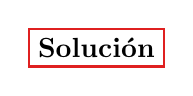
\begin{tikzpicture}[outline/.style={draw=red!75!gray,thick,fill=white!80!white}]
    \node [outline=red] at (0,1) {\bf Solución \\};
    \end{tikzpicture}\\}
    }
\end{comment}
%%%%%%%%%%%%%%%%%%%%%%%%%%%%%%%%%%%%%%%%%%%%%%%%%%%%%%%%%%%%%%%%%%%%%%%%%%%%%%

%Notas extra.
%%%%%%%%%%%%%%%%%%%%%%%%%%%%%%%%%%%%%%%%%%%%%%%%%%%%%%%%%%%%%%%%%%%%%%%%%%%%%%
\begin{comment}
    Notas:
    
    %Inserción de referencias. Acordeón de BibLaTeX.
    Cheet sheat: http://tug.ctan.org/info/biblatex-cheatsheet/biblatex-cheatsheet.pdf
    
    %Inserción de referencias. BibTeX. Al final del archivo principal, colocar
    \bibliography{fuentes}
    
    %Inserción de algún .pdf. Agregar el siguiente comando donde se quiere insertar archivo.
    \includepdf[page={-}]{pdf name}
    
    %Inserción de código (programación). Agregar el siguiente comando donde se quiere insertar código.
    \begin{lstlisting}[language=Python]
        Código.
    \end{lstlisting}
    
    %Inserción de archivo código (programación). Colocar al final de "main.tex".
    \lstinputlisting[language=Python,fisrtline=1,lastline=12]{Codigo.py}
    
    %Edición de diapositivas. Acordeón de Beamer.
    Cheat sheat: http://nikhildamodaran.weebly.com/uploads/3/8/0/9/38095403/beamer-appearance-cheat-sheet.pdf
\end{comment}
%%%%%%%%%%%%%%%%%%%%%%%%%%%%%%%%%%%%%%%%%%%%%%%%%%%%%%%%%%%%%%%%%%%%%%%%%%%%%%

%Estilo del código (programación) para insertar en LaTeX.
%%%%%%%%%%%%%%%%%%%%%%%%%%%%%%%%%%%%%%%%%%%%%%%%%%%%%%%%%%%%%%%%%%%%%%%%%%%%%%
\definecolor{codegreen}{rgb}{0,0.6,0}
\definecolor{codepurple}{rgb}{0.6,0.2,0.8}
\definecolor{codegray}{rgb}{0.5,0.5,0.5}
\definecolor{codered}{rgb}{0.7,0.13,0.13}
\definecolor{backcolour}{rgb}{0.96,0.96,0.96}
\lstdefinestyle{mystyle}{
    backgroundcolor=\color{backcolour},   
    commentstyle=\color{codegreen},
    keywordstyle=\color{codepurple},
    numberstyle=\tiny\color{codegray},
    stringstyle=\color{codered},
    basicstyle=\ttfamily\footnotesize,
    breakatwhitespace=false,
    breaklines=true,                 
    captionpos=b,                    
    keepspaces=true,                 
    numbers=left,                    
    numbersep=5pt,                  
    showspaces=false,                
    showstringspaces=false,
    showtabs=false,                  
    tabsize=2
}
\lstset{style=mystyle}
%%%%%%%%%%%%%%%%%%%%%%%%%%%%%%%%%%%%%%%%%%%%%%%%%%%%%%%%%%%%%%%%%%%%%%%%%%%%%%

%Operadores y símbolos matemáticos.
%%%%%%%%%%%%%%%%%%%%%%%%%%%%%%%%%%%%%%%%%%%%%%%%%%%%%%%%%%%%%%%%%%%%%%%%%%%%%%
\DeclareMathOperator*{\Res}{Res} %\Res_{ #1 }{ #2 } Residuo.
\DeclareMathOperator{\Lapt}{\mathscr{L}} %\Lapt{ #1 } Transformada de Laplace.
\DeclareMathOperator{\Four}{\mathscr{F}} %\Four{ #1 } Transformada de Fourier.
\DeclareMathOperator{\Gammaf}{\Gamma} %\Gammaf{ #1 } Función Gamma.
\DeclareMathOperator{\betaf}{\beta} %\Betaf{ #1 } Función beta.
\DeclareMathOperator{\erf}{erf} %\erf{ #1 } Función error.
\DeclareMathOperator{\erfc}{erfc} %\erfc{ # } Función error complementaria.
\newcommand{\oo}{\infty} %\oo Infinito.
\newcommand{\C}{\mathbb{C}} %\C Conjunto de los complejos.
\newcommand{\R}{\mathrm{I}\!\mathrm{R}} %\R Conjunto de los reales.
\newcommand{\Q}{\mathbb{Q}} %\Q Conjunto de los racionales.
\newcommand{\Z}{\mathbb{Z}} %\Z Conjunto de los enteros.
\newcommand{\N}{\mathrm{I}\!\mathrm{N}} %\N Conjunto de los naturales.
\newcommand{\dbar}{d\mkern-7mu\mathchar'26\mkern-2mu} %\dbar Diferencial de función de proceso.
\newcommand{\Ham}{\mathcal{H}} %\Ham{ #1 } Hamiltoniano.
\newcommand{\Lag}{\mathcal{L}} %\Lag{ #1 } Lagrangiano.
\newcommand{\Par}[1]{\left( #1 \right)} %\Par{ #1 } Paréntesis.
\newcommand{\Sqbr}[1]{\left[ #1 \right]} %\Sqbr{ #1 } Corchetes (square brackets)
\newcommand{\Braces}[1]{\left\{ #1 \right\}} %\Braces{ #1 } Llaves.
\newcommand{\Abs}[1]{\left| #1 \right|} %\Abs{ #1 } Valor absoluto.
\newcommand{\Mean}[1]{\langle #1 \rangle} %\Mean{ #1 } Valor esperado.
\newcommand{\Bra}[1]{\left\langle #1 \right|} %\Bra{ #1 } Bra en notación de Dirac.
\newcommand{\Ket}[1]{\left| #1 \right\rangle} %\Ket{ #1 } Ket en notación de Dirac.
\newcommand{\Braket}[2]{\left\langle#1\right|\left.#2\right\rangle} %\Braket{ #1 }{ #2 } Bra-Ket en notación de Dirac.
\newcommand{\Div}[2]{\nabla{#1}\cdot{#2}} %\Div{ #1 }{ #2 } Divergencia.
\newcommand{\Curl}[2]{\nabla{#1}\times{#2}} %\Curl{ #1 }{ #2 } Rotacional.
\newcommand{\Grad}[2]{\nabla{#1}{#2}} %\Grad{ #1 }{ #2 } Gradiente.
\newcommand{\Lap}[2]{\nabla{#1}^2{#2}} %\Lap{ #1 }{ #2 } Laplaciano.
\newcommand{\System}[1]{\left\{ {#1} \right.}
%\System{ #1 } Remarca un sistema de ecuaciones con una llave. Se usa junto con la función array.
\newcommand{\Def}[3]{\left. {#1} \right|_{#2}^{#3}} 
%\Def{ #1 }{ #2 }{ #3 } Determina los límites a evaluar de la expresión dada.
\newcommand{\D}[3]{\dfrac{d^{#1}}{d{#3}^{#1}}#2}
%\D{#Orden}{#Función}{#Variable indep.} Derivada de orden n. Si es de orden 1, no se anota el primer argumento. La función aparece fuera del operador
\newcommand{\Df}[3]{\dfrac{d^{#1}#2}{d{#3}^{#1}}}
%\D{#Orden}{#Función}{#Variable indep.} Derivada de orden n. Si es de orden 1, no se anota el primer argumento. La función aparece dentro del operador
\newcommand{\Dpartial}[3]{\dfrac{\partial^{#1}}{\partial{#3}^{#1}}#2}
%\Dpartial{#Orden}{#Función}{#Variable indep.} Derivada parcial de orden n. La función aparece fuera del operador
\newcommand{\Dfpartial}[3]{\dfrac{\partial^{#1}#2}{\partial{#3}^{#1}}} %\Dpartial{#Orden}{#Función}{#Variable indep.} Derivada parcial de orden n. La función aparece dentro del operador.
\newcommand{\Dpartialcruz}[3]{\dfrac{\partial^{2}}{\partial{#2}\partial{#3}}{#1}}
%\Dpartialcruz{#Función}{#Variable_1 indep.}{#Variable_2 indep.} Derivada parcial de orden 2 cruzada. La función aparece fuera del operador
\newcommand{\Dfpartialcruz}[3]{\dfrac{\partial^{2}#1}{\partial{#2}\partial{#3}}}
%\Dfpartialcruz{#Función}{#Variable_1 indep.}{#Variable_2 indep.} Derivada parcial de orden 2 cruzada. La función aparece dentro del operador
%%%%%%%%%%%%%%%%%%%%%%%%%%%%%%%%%%%%%%%%%%%%%%%%%%%%%%%%%%%%%%%%%%%%%%%%%%%%%%

\author{Santiago Alberto Flores Román}                  % Nombre del autor
\title{Entropía informacional de átomos: Implementación del método de integración numérica Las Vegas+}         % Título de la tesis
\asesor{Dr. Juan Manuel Solano Altamirano\\
        Dr. Jorge Velázquez Castro}               % Nombre de los asesores
\presidente{Dr. Eduardo Moreno Barbosa} % Nombre del presidente del jurado
\secretario{Dr. Javier Miguel Hernández López}       % Nombre del secretario del jurado
\vocala{Dr. Julio Manuel Hernández Pérez}         % Nombre del 1er vocal del jurado
\vocalb{Dra. Beatriz Bonilla Capilla}                   % Nombre del 2do vocal del jurado
%\vocalc{}                         % Nombre del 3er vocal del jurado
                                   % Usarse sólo si se hizo \include{parche}

\date{\today}                      % Fecha del examen profesional.
                                   % Escribirse en el formato mes año:
                                   % por ejemplo \date{Julio de 2018}

\hombre
% \mujer       %----Es una mujer quien escribe su trabajo
%tesina      %----En caso de escribir una tesina.

\begin{document}
\frontmatter
           \portada         %----quitar comentario en la versión final
           \maketitle       %----quitar comentario en la versión final
           \makeacta        %----quitar comentario en la versión final
           \setcounter{page}{4}		% La primer página con número impreso
           							% debe ser la siguiente al acta (pág. impar)
           							% pero el conteo se hace a partir del
           							% maketitle, (segunda portada)	
          							% El valor 4 puede cambiarse según corresponda.
           \chapter*{}
\vspace{5cm}

\begin{flushright}
{\fontfamily{pzc}\fontsize{15}{1}\selectfont{
    Mira la cumbre de la montaña, pero recuerda admirar las cosas bellas del camino sin olvidar los pasos que dejas atrás.\\
    Después de todo, el regalo es la experiencia y la cima es parte del viaje.
    \\ \vspace{0.5cm}
    {\em Santiago Flores}}}
\end{flushright}

\chapter*{Dedicatoria}
    Para mi amada esposa Diana Marlén y mis queridos abuelos, a quienes llevaré siempre en mi corazón.

\chapter*{Agradecimientos}
    Aquí van los agradecimientos

           \tableofcontents %----quitar comentario en la versión final

\mainmatter  % A partir de aquí va el trabajo propio, se hará colocando
             % comandos \include{archivo} donde archivo es el nombre de 
             % un archivo de latex con nombre "archivo.tex"
             % Notar que en sistemas Unix las mayúsculas son diferentes
             % a las minúsculas.
\addcontentsline{toc}{chapter}{Resumen}
\chapter*{Resumen}
    \noindent En este trabajo se estudia la entropía de la información de Shannon en un conjunto de átomos en su estado base. Se busca establecer la posible aplicación de la entropía de Shannon como una medida de la calidad de la descripción de la densidad electrónica. Para esto, se calculan las densidades electrónicas de los átomos utilizando diversas bases y métodos de la química computacional. La entropía de Shannon se obtiene a través de una integración numérica con el método Las Vegas+. Parte importante del trabajo consiste en la implementación eficiente de este algoritmo, además de adaptarlo a la suite \textit{DensToolKit}, el cual está programado en C++ y es un código libre.
    
\chapter{Introducción}
    \noindent Dos de los conceptos medulares en la química computacional son la función de onda y la densidad electrónica, pues estas dos albergan toda la información electrónica del sistema, ya sea átomo o molécula, y el conocimiento de su comportamiento electrónico permite describir las causas y consecuencias de la formación y rompimiento de enlaces. Incluso, su importancia ha incitado a que varios autores hayan desarrollado programas o paquetes, como \textit{DensToolKit}, que se enfocan en calcular la densidad electrónica de un sistema específico y realizar diversos análisis con ella misma.
    
    Uno de los problemas presentes en la química computacional es que la única manera hasta ahora conocida de aproximarse a la función de onda de un átomo o molécula es a través de métodos numéricos como Hartree-Fock (HF) o los métodos perturbativos M\o ller-Plesset, los cuales son MP2(full), MP3(full), MP4(SDQ), entre otros. La manera en que se utilizan los métodos para describir el comportamiento electrónico de átomos es primero componiendo funciones de onda llamadas orbitales moleculares, conformadas por combinaciones lineales de funciones monoelectrónicas llamadas orbitales atómicos que aproximen el estudio del sistema a una superposición de diversos átomos hidrogeoides, cuyas soluciones pueden conocerse al resolver la ecuación de Schr\"odinger para cada orbital mencionado. Una manera de componer tales orbitales atómicos es a través de combinaciones lineales de funciones llamadas funciones primitivas y algunos ejemplos de estos son 6-31G, 6-31+G**, 6-31G(2df,p), aug-cc-pVDZ o aug-cc-pVTZ, a los cuales uno puede acceder a través de programas como Gaussian09 \cite{gaussian09}. Estos son conjuntos de funciones de tipo gaussiano que al superponerse se asemejan a los orbitales atómicos.
    
    Respecto a la densidad electrónica, su utilización surge por el desarrollo de la Teoría del Funcional de la Densidad (DFT por sus siglas en inglés), cuyo problema radica en el desconocimiento del funcional de la energía de correlación e intercambio ($E_{CX}$) en la mayoría de los sistemas conocidos. No obstante, varios autores han sugerido aproximaciones a partir del acompañamiento de parámetros experimentales y de sistemas conocidos como un gas de electrones uniforme, donde este funcional sí se conoce y a volúmenes infinitesimales su comportamiento se asemeja a una mayor variedad de sistemas. Los funcionales B3LYP y $\omega$B97X-D presentan esas características y también son accesibles a través de Gaussian09. Respecto a la densidad electrónica, esta puede calcularse a través de los mismos conjuntos de funciones base mencionados en el párrafo anterior. Cabe mencionar que los funcionales en DFT habrán de depender esencialmente de la densidad electrónica.
    
    Además del funcional de la energía de correlación e intercambio, existe una gran variedad de funcionales y uno de ellos es la entropía de Shannon, la cual también llamaremos en la presente como entropía informacional. Este objeto es de interés en la química computacional debido a varias razones, pero en la tesis presente, el enfoque se encuentra en que ha sido sugerida para medir la calidad de los conjuntos de funciones base, haciendo referencia a <<calidad>> como las aproximaciones de los efectos de la función de onda calculada numéricamente con respecto a las observaciones experimentales. A pesar de que varios autores han estado estudiando esta utilidad \cite{sagar,ho,tripathi,gadre}, hasta ahora no se ha logrado concluir si esta es determinante para la medida de la calidad mencionada.
    
    Por último, es importante mencionar que la teoría DFT tiene la dificultad de que la densidad electrónica presenta desde uno a varios centros cuasi-singulares que complican su integración y hay funcionales que no son fáciles de conocer hasta el presente. Por consiguiente, no sería fácil utilizarlos como integrandos, tal como sucede con la entropía de Shannon. Entonces se vuelve necesario el uso de métodos de integración que no requieran previo conocimiento del comportamiento del integrando, como el método de integración Monte Carlo o sus derivados como Las Vegas+, método que se basa principalmente en el muestreo de importancia.
    
    En la tesis presente se mencionará la implementación del algoritmo de integración Las Vegas+ en el paquete de programas \textit{DensToolKit} para probar si la entropía informacional es útil para medir la calidad de conjuntos de funciones base, de los cuales se utilizaron los mencionados al principio de este capítulo. Los sistemas de estudio fueron el conjunto de átomos del hidrógeno al kriptón y los métodos y funcionales utilizados también fueron los mencionados arriba.
    
\chapter{Objetivos}
    \section{General}
        Implementar el método de integración numérico Monte Carlo, en su variante Las Vegas+, y adaptarlo al programa DensToolKit, con el fin de estudiar las entropías informacionales de átomos y moléculas.
    \section{Específicos}
        \begin{itemize}
            \item Implementar el método Vegas-Monte Carlo para realizar integrales numéricas 3D de funciones con varios centros cuasi-singulares.
            \item Incorporar el método en el software DensToolKit.
            \item Analizar la entropía informacional en un conjunto de átomos en su estado base (del Hidrógeno al Criptón), con diferentes bases y métodos.
            \item Analizar la entropía informacional en un conjunto pequeño de moléculas, las cuales tienen 10 electrones en total, con diferentes bases y métodos.
        \end{itemize}
\chapter{Antecedentes}
    \section{DensToolKit}
        \noindent \textit{DensToolKit} es un paquete de programas con licencia GNU-GPLv3 y desarrollados por \textit{Solano-Altamirano, J. M. y Hernández-Pérez J. M.} \cite{manuel} enfocados en analizar densidades electrónicas y varios campos derivados de ellos, tales como el gradiente de la densidad electrónica, la función de localización electrónica (ELF por sus siglas en inglés) junto con su gradiente, región de electrones lentos (RoSE por sus siglas en inglés), gradiente de densidad reducida, detector de electrones localizados (LED por sus siglas en inglés), entropías de la información, potencial electrostático, densidades $K$ y $G$ de energía cinética, entre otros, incluso en el espacio de momentos. Además, también incluye programas que se encargan de ubicar puntos críticos y enlaces químicos, todo en moléculas y átomos, usando como referencia la teoría cuántica de átomos en moléculas (QTAIM por sus siglas en inglés). 
        Algunos de sus programas son
        \begin{itemize}
            \item dtkpoint, el cual evalúa los campos implementados en un punto o en un conjunto de puntos, y
            \item dtkbpdens, cuya tarea es evaluar uno de los campos implementados a lo largo del trayecto del enlace entre dos átomos.
        \end{itemize}
        
        DensToolKit solicita como entrada archivos de formato \textit{wfn} ó \textit{wfx}, los cuales son producidos por programas tales como Gamess, NWChem, MOLPRO o Gaussian. Tales archivos contienen la expansión de la función de onda molecular o atómica en términos bases gaussianas. 
        
        No obstante la variedad de sus programas, no hay uno que se encargue de integrar los campos escalares mencionados, por lo que es necesario implementar en él un algoritmo de integración para integrar cualquiera de los campos que ofrezca la suite.
    
    \section{Método Monte Carlo}
        \noindent Dada una función $f:\R^d\rightarrow\R$, con $d\in\N$, se puede encontrar su integral sobre un volumen $\Omega\in\R^d$ utilizando $N_{ev}$ puntos aleatorios generados a partir de una densidad de probabilidad arbitraria $p(\bm{x})$, con $\bm{x}\in\R^d$. Numéricamente, es
        \begin{align}
            \Mean{f^l} = \frac{1}{N_{ev}}\sum_{N_{ev}}\Par{\frac{f(\bm{x})}{p(\bm{x})}}^l,
        \end{align}
        siendo $I$ la integral exacta de $f$ sobre el volumen $\Omega$, $l\in\N$ y de modo que $\Mean{f}\rightarrow I$ cuando $N_{ev}\rightarrow\oo$.
        
        Su varianza se puede determinar a partir de la expresión
        \begin{align}\label{eq: devest mc}
            \sigma^2 = \frac{\Mean{f^2}-\Mean{f}^2}{N_{ev}-1}
        \end{align}
        y consecuentemente, su desviación estándar es
        \begin{align}
            \sigma = \sqrt{\frac{\Mean{f^2}-\Mean{f}^2}{N_{ev}-1}}.
        \end{align}
        
        La ecuación \eqref{eq: devest mc} muestra la tendencia hacia la integral $I$ conforme incrementan los puntos de muestreo que se realizan sobre $\Omega$. Esta tendencia puede resultar costosa en rendimiento computacional al ralentizarse a un ritmo de
        \begin{align}
            \sqrt{\frac{1}{N_{ev}}},
        \end{align}
        es por eso que se han desarrollado métodos adaptativos que buscan reducir ese costo sin sacrificar las ventajas del mismo método.
        
        \subsection{\textit{Muestreo de importancia}}
            \noindent La varianza $\sigma^2$ puede reducirse hasta alcanzar un valor óptimo, el cual es
                \begin{align}\label{eq: densidad optima}
                    p(\bm{x}) = \frac{\Abs{f(\bm{x})}}{\int_{\Omega}\Abs{f(\bm{x})}}.
                \end{align}
            Aunque en la práctica es imposible alcanzarlo, la ecuación \eqref{eq: densidad optima} muestra que tal valor se logra cuando las evaluaciones sobre $f$ se concentran en donde su magnitud es mayor.
            
        \subsection{\textit{Muestreo estratificado}}
            \noindent Uno de los métodos para alcanzar la varianza $\sigma^2$ óptima es subdividiendo la región $\Omega$ en $N_g$ subconjuntos $\omega_i$, con $i\in\{1,2,\dots,N_g\}$, de tamaño variable, llamados incrementos. De ese modo, se puede integrar utilizando $N_{ev}/N_g$ puntos de muestreo aleatorios en cada $\omega_i$.
                
            La varianza utilizando este método, $\sigma_s^2$, puede reducirse hasta un valor
            \begin{align}
                \sigma_s^2 \rightarrow \frac{\sigma^2}{N_g},
            \end{align}
            sin embargo el número de evaluaciones sobre $f$ crece al valor $N_{ev}=2N_g^d$, volviéndose un serio problema cuando se trata de integrales en múltiples dimensiones.
        
    \section{Método Las Vegas+}
        \noindent A este método de integración también lo llamaremos Las Vegas-Monte Carlo y fue desarrollado por primera vez por \textit{Lepage, P.} \cite{lepage1978} en 1978. Este método ha sido ampliamente utilizado que incluso llegó a usarse en el CERN \cite{vegas-cern} y se implementó en diversos lenguajes de programación como en Fortran \cite{lepagefortran} o Python a través del programa VegasFlow \cite{vegasflow}. Además, se propusieron mejoras de la primera versión por parte de otros desarrolladores \cite{vegas-revisited} para el área de la física de partículas. La última mejora implementada sobre este método fue publicada por su propio autor en agosto del 2021 y lo llamó Las Vegas+ \cite{lepage2021}.
        
        La importancia de este método iterativo radica en su capacidad de adaptarse al integrando para reducir la incertidumbre $\sigma^2$ prontamente, disminuyendo el número de evaluaciones a un orden $O(N_gd)$, en lugar de $O\Par{N_g^d}$, donde $N_g$ y $d$ son el número de incrementos y de dimensiones, respectivamente.
        
        Dada una una función $f$ continua en un intervalo $(a,b)$, su integral puede obtenerse a través de un remapeo que la exprese en el intervalo $(0,1)$,
        \begin{align}
            I = \int_a^bdxf(x) \Rightarrow T = \int_0^1dyJ(y)f(x(y)),
        \end{align}
        donde $J$ es el jacobiano de la transformación. Para su aplicación en la computación, la segunda integral puede obtenerse a través de una aproximación discreta, es decir,
        \begin{align}
            I \approx S = \frac{1}{N_{ev}}\sum_yJ(y)f(x(y)),
        \end{align}
        donde $N_{ev}$ es el número de evaluaciones que se realizan sobre $f$.
        
        En términos estadísticos, la integral $I$ es el valor esperado de la muestra de puntos obtenidos a través de una distribución aleatoria uniforme, por lo que la incertidumbre que presenta este método de integración es
        \begin{align}
            \sigma^2 = \frac{1}{N_{ev}-1}\Par{\sum_y\Sqbr{J(y)}^2\Sqbr{f(x(y))}^2-S^2}
        \end{align}
        
        Se escoge tal transformación para minimizar la incertidumbre al integrar a través del método Monte Carlo y además se genera un mallado en el espacio original que varía en su forma (pero no en tamaño), de modo que
        \begin{align*}
            x_0 & = a\\
            x_1 & = x_0+\Delta x_0\\
            & \cdots\\
            x_{N_g} & = x_{N_g-1}+\Delta x_{N_g-1} = b.
        \end{align*}
        Tal mallado permite determinar la transformación, la cual es
        \begin{align}
            x(y) & = x_{i(y)}+\Delta x_{i(y)}\delta(y),
        \end{align}
        donde $i(y)$ y $\delta(y)$ son las partes entera y fraccionaria de $yN_g$, respectivamente,
        \begin{align}
            i(y) & \equiv floor(yN_g),\\
            \delta(y) & \equiv yN_g-i(y),
        \end{align}
        con $y = i/N_g$ en el punto $x_i$. Así mismo, el jacobiano es
        \begin{align}
            J(y) = N_g\Delta x_{i(y)},
        \end{align}
        el cual es una función escalonada con anchos $\Delta x_i$.
        
        Otra ventaja de la transformación mencionada es la manera en que trata al integrando en el nuevo espacio, pues concentra el muestreo de puntos en aquellas zonas del integrando donde se presenten picos pronunciados y reduce el muestreo en zonas donde el integrando sea plano. En promedio, cada intervalo recibirá un mismo número de puntos de muestreo (alrededor de $N_{ev}/N_g$), mostrando la aplicación del muestreo de importancia como método adaptativo en Monte Carlo.
        
        El procedimiento del método Las Vegas+ consiste en generar un mallado uniforme y realizar un muestreo Monte Carlo para adquirir información del integrando, la cual será usada para modificar el mallado y realizar nuevamente un muestreo. Sucesivamente, el algoritmo recaudará cada vez más información para al final alcanzar un mallado óptimo y adaptado al comportamiento de la función a integrar.
        
        La herramienta que extraerá información del integrando es
        \begin{align}
            d_i \equiv \frac{1}{n_i}\sum_{x(y)\in\Delta x_i}\Sqbr{J(y)}^2\Sqbr{f(x(y))}^2,
        \end{align}
        el cual deberá tender a una constante como índice de un mallado óptimo. Para realizar el refinamiento del mallado, $d_i$ debe redefinirse como
        \begin{align}
            d_i \rightarrow \Par{\frac{1-d_i}{\ln{\Sqbr{1/d_i}}}}^{\alpha},
        \end{align}
        donde $\alpha$ se define como taza de convergencia y su valor depende del integrando, obteniéndose a prueba y error. Sin embargo, típicamente se escoge $\alpha=1$ y el valor $\alpha=0$ indica que ya no se realizará más refinamiento del mallado. Este parámetro es una constante durante el proceso de integración.
        
        Para saber si $d_i$ es constante, se busca que en cada intervalo $d_i$ sea considerablemente igual. Sean
        \begin{align}\label{eq: d d_i}
            d & \equiv \sum_i d_i \nonumber\\
            \text{y} & \\
            \delta d & \equiv \frac{\sum_id_i}{N_g}. \nonumber
        \end{align}
        Una vez definidas las variables \eqref{eq: d d_i}, se procede al siguiente algoritmo.
        \begin{enumerate}
            \item Se inicializan las variables siguientes.
                \begin{align*}
                    x_0' & = x_0\\
                    x_{N_g}' & = x_{N_g}\\
                    i & = 0\;\text{(índice del mallado $x'$)}\\
                    j & = 0\;\text{(índice del mallado $x$)}\\
                    S_d & = 0\;\text{(Cantidad de $d$ acumulada)}
                \end{align*}
            \item Se incrementa $i$ una unidad. Si $i\ge N_g$, el nuevo mallado ya terminó de generarse.
            \item Se procede al siguiente paso si $S_d \ge \delta d$; de otro modo, se agrega $d_j$ a $S_d$ y se incrementa $j$ una unidad, volviendo al paso anterior.
            \item Restamos $\delta d$ a $S_d$ y se calculan los límites del nuevo intervalo por interpolación:
                \begin{align}
                    x_i' = x_j - \frac{S_d}{d_{j-1}}\Delta x_{j-1}.
                \end{align}
                Se regresa al paso 2.
        \end{enumerate}
        
        Una vez generada la nueva malla, se reemplaza la anterior por esta, se realiza un nuevo muestreo Monte Carlo y se repite el procedimiento hasta alcanzar el mallado óptimo y que el estimado de la integral sea suficientemente preciso.
        
        Para funciones cuyo dominio se encuentre en un espacio multidimensional, es decir,
        \begin{align}
            I = \int_0^1d^DyJ(y)f(\bm{x}(y)),
        \end{align}
        donde $D$ representa el número de dimensiones que componen al espacio, los cambios que se hacen son
        \begin{align}
            d_i^\mu \equiv \frac{1}{n_i^{\mu}}\sum_{x^{\mu}(y^{\mu})\in\Delta x_i^{\mu}}\Sqbr{J(y)}^2\Sqbr{f(\bm{x}(y))}^2,
        \end{align}
        donde $\mu$ representa la dimensión respectiva, $0<y^{\mu}<1$ y
        \begin{align}
            J(y) = \prod_{\mu} J^{\mu}(y).
        \end{align}
        
        Dado que cada integración Monte Carlo arroja información sobre el integrando, se puede utilizar también para obtener un estimado acumulado y una varianza acumulada que ayudan a amortiguar la variación de ambas estimaciones, las cuales se pueden determinar mediante
        \begin{align}
            \bar{I} & = \frac{\sum_jI_j/\sigma_j^2}{\sum_j1/\sigma_j^2} \nonumber\\
            \text{y} & \\
            \sigma_{\bar{I}} & = \Par{\sum_j\frac{1}{\sigma_j^2}}^{-1/2}, \nonumber
        \end{align}
        siendo $j$ el índice del número de iteraciones.
        
        Por último, se debe verificar que los resultados obtenidos en cada iteración sean consistentes con respecto a las incertidumbres estimadas. La forma de hacerlo es a través de pruebas $\chi^2$, expresadas para este caso como
        \begin{align}
            \chi^2 = \sum_j\frac{\Par{I_j-\bar{I}}^2}{\sigma_j^2}.
        \end{align}
        
        Si $\chi^2$ llegara a ser mayor al número de iteraciones presentes (menos uno), el proceso de integración deberá reiniciarse.
        
        Hay casos donde $\chi^2$ supera con frecuencia el umbral mencionado anteriormente. Algunas veces se debe a que la malla no se encuentra lo suficientemente refinada en las primeras iteraciones y otras veces a que el número de puntos de muestreo no es lo suficientemente grande para garantizar un comportamiento gaussiano alrededor de la integral. Para solucionar el primero, se puede eliminar la estimación obtenida en las primeras iteraciones (termalización) para considerar solo aquellas donde el mallado ya se encuentra lo suficientemente refinado; para el segundo caso, será suficiente con incrementar el número de puntos de muestreo a utilizar por iteración.
        
    \section{Entropía de Shannon}
        \noindent Este concepto, desarrollado por \textit{Shannon, C. E.} \cite{shannon2001} y nombrado como tal por su autor debido a su semejanza con la entropía definida en la mecánica estadística, se encarga de medir la cantidad de desinformación que presenta una variable aleatoria y matemáticamente se define como
        \begin{align}
            H(p_1,p_2,\dots,p_n) \equiv -K\sum_{i=1}^np_i\log{p_i},
        \end{align}
        donde $p_i(x)=P\Par{X=x_i}$, con $X$ asociada al conjunto $\mathbb{X}$, es la probabilidad de ocurrencia de un evento $i$-ésimo, $K$ es una constante positiva y se define $p_i\log{p_i} \equiv 0$ cuando $p_i(x)=0$. O bien, dado $p(x)=P(X=x)$, la entropía de Shannon también puede expresarse como
        \begin{align}\label{eq: shannon varal}
            H(X) = -K\sum_{x\in \mathbb{X}}p(x)\log{\Sqbr{p(x)}}.
        \end{align}
    
        También existe la entropía para variables aleatorias conjuntas \cite{thomas_entropy}. Dadas dos variables aleatorias $X$ y $Y$ con probabilidad conjunta $p(x,y)=P\Par{X=x,Y=y}$ y conjuntos $\mathbb{X}$ y $\mathbb{Y}$, la entropía conjunta se define como
        \begin{align}
            H(X,Y) \equiv -K\sum_{x\in\mathbb{X}}\sum_{y\in\mathbb{Y}}p(x,y)\log{\Sqbr{p(x,y)}},
        \end{align}
        mientras que para variables condicionales, la entropía condicional es
        \begin{align}
            H(Y|X) & = \sum_{x\in\mathbb{X}}p(x)H(Y|X=x) \nonumber\\
            & = -K\sum_{x\in\mathbb{X}}p(x)\sum_{y\in\mathbb{Y}}p(y|x)\log{\Sqbr{p(y|x)}}.
        \end{align}
        
        $H$ satisface las siguientes propiedades:
        \begin{enumerate}
            \item $H$ es continua en cada probabilidad $p_i$, con $i=1,2,\dots,n$.
        
            \item Si todas las probabilidades son iguales, $p_i=1/n$, siendo $n$ el número de eventos posibles, entonces $H$ es una función monótona creciente y dependiente de $n$. Para probabilidades distintas, $H\leq \log{n}$. Esto quiere decir que los eventos con la misma probabilidad de ocurrir, tienen más incertidumbre cuando hay un mayor número de eventos posibles.
        
            \item $H(p_i)\geq 0$ cuando $0 \leq p_i \leq 1$. En caso de que $H(p_i) = 0$, el evento $i$-ésimo será seguro.
        
            \item La entropía de Shannon también se puede interpretar como un valor esperado:
                \begin{align}
                    H(X) = K\Mean{\log{\Par{1/p(x)}}}_X,
                \end{align}
                donde el operador $\Mean{\cdot}_X$ hace referencia al valor esperado de la variable aleatoria $X$.\\
                Para variables conjuntas,
                \begin{align}
                    H(X,Y) = -K\Mean{\log{\Sqbr{p(x,y)}}}_{XY},
                \end{align}
                y para variables condicionales,
                \begin{align}
                    H(Y|X) = -K\Mean{\log{\Sqbr{p(Y|X)}}}_{XY}.
                \end{align}
        
            \item La entropía de un par de variables aleatorias es la entropía de la una más la entropía condicional de la otra, es decir,
                \begin{align}
                    H(X,Y) = H(X)+H(X|Y).
                \end{align}
        
            \item La incertidumbre de dos variables conjuntas siempre será menor a la suma de las incertidumbres individuales, a menos que las segundas sean independientes.
            \begin{align}\label{eq: desigualdad triangulo}
                H(X,Y) \leq H(X)+H(Y).
            \end{align}
            Esto quiere decir que la mínima incertidumbre que se puede alcanzar ocurre cuando los eventos son independientes entre sí.
            También se cumple que
            \begin{align}
                H(X) \geq H(X|Y)
            \end{align}
            y nuevamente la igualdad se alcanza cuando ambas variables son independientes entre sí.
        \end{enumerate}
    
        \subsection{Entropía relativa}
            \noindent Más allá de las entropías mencionadas anteriormente, existe la entropía relativa o distancia \textit{Kullback Leibler} entre dos funciones de masa de probabilidad $p(x)$ y $q(x)$ normalizadas a 1 \cite{thomas_entropy}, la cual se define como
            \begin{align}
                H(p||q) \equiv \sum_{x\in X}p(x)\log{\Sqbr{\frac{p(x)}{q(x)}}} = \Mean{\log(p/q)}_X.
            \end{align}
            
            También se ha de definir $H(p||q) \equiv 0$ cuando $p=0$, y cumple propiedades semejantes a su análoga absoluta, por ejemplo:
            \begin{align}
                H\Par{p||q} \geq 0
            \end{align}
            y se alcanzará la igualdad si y solo si $p(x) = q(x),\forall x\in X$.
        
            La entropía relativa $H(p||q)$ representa la distancia entre las masas de probabilidad $p$ y $q$, tomando a $q$ como referencia.
        
            Por último, las mismas entropías mencionadas en toda la sección tienen su equivalencia para densidades de probabilidad. Estas son
            \begin{align}
                H(x) & = -K\int_{x\in X} p(x)\log{\Sqbr{p(x)}}dx, \nonumber\\
                H(x,y) & = -K\int_{x\in X}\int_{y\in Y}p(x,y)\log{\Sqbr{p(x,y)}}dydx \nonumber\\
                \text{y} & \\
                H(p||q) & = \int_{x\in X}p(x)\log{\Sqbr{\frac{p(x)}{q(x)}}}dx, \nonumber
            \end{align}
            para variables aleatorias continuas.
        
        \subsection{Aplicación de la entropía de Shannon en átomos y moléculas}
            \noindent La densidad electrónica de un átomo o molécula, comúnmente expresada como $\rho(\bm{r})$ y definida como
            \begin{align}\label{eq: densidad elec}
                \rho(\bm{r}) \equiv N_{e}\int d\sigma_1d\bm{x}_2\cdots d\bm{x_N}\psi^*\Par{\bm{x}_1,\bm{x}_2,\dots,\bm{x}_N}\psi\Par{\bm{x}_1,\bm{x}_2,\dots,\bm{x}_N},
            \end{align}
            donde $\bm{x}_i=x(\bm{r}_i,\sigma_i)$, $\sigma_i$ es el espín del $i$-ésimo electrón y $N_{e}$ es el número de electrones que componen al átomo o la molécula, alberga la información del número de electrones por unidad de volumen en un punto del espacio de posiciones \cite{jensen}. Cabe notar que se considera un espacio 4-dimensional (por cada electrón) sobre $\psi$ al ser esta una función antisimétrica, por lo que el espín influye considerablemente en la localización de los electrones sobre el espacio 3-dimensional. Así mismo, la densidad electrónica puede estudiarse tanto en el espacio de posiciones, como en el espacio de momentos a través de la transformada de Fourier, y su expresión es $\Pi=\Pi(\bm{p})$. Esto debido a que el espacio es Fourier es el espacio de momentos:
            
            \begin{align}
                \Pi(\bm{p}) = \frac{1}{(2\pi)^{3/2}}\int\rho(\bm{r})e^{-i\bm{p}\cdot\bm{r}}d\bm{r},
            \end{align}
            en unidades atómicas.
        
            A sabiendas de la utilidad de la función \eqref{eq: densidad elec}, la entropía de Shannon puede otorgar información sobre el grado de localización de los electrones en un átomo o molécula: Cuanto mayor sea su valor, mayor incertidumbre habrá sobre sus posiciones o cantidades de movimiento. Conocida la densidad electrónica de un átomo o molécula, las entropías de Shannon en el espacio de posiciones $S_{\rho}$ y en espacio de momentos $S_{\Pi}$ pueden expresarse como \cite{sagar}
            \begin{align}\label{eq: entropia N}
                S_{\rho}^{N_{e}}(\bm{r}) & = -\int\rho\!\Par{\bm{r}}\ln{\Sqbr{\rho\!\Par{\bm{r}}}}d\bm{r} \nonumber\\
                \text{y} & \\
                S_{\Pi}^{N_{e}}(\bm{p}) & = -\int\Pi\!\Par{\bm{p}}\ln{\Sqbr{\Pi\!\Par{\bm{p}}}}d\bm{p}. \nonumber
            \end{align}
            
            Cabe remarcar que en ambas ecuaciones, las densidades no se encuentran normalizadas a 1. En tal caso, pasarán a ser \cite{sagar}
            \begin{align}\label{eq: entropia 1}
                S_{\rho}^1(\bm{r}) & = -\int\frac{\rho\!\Par{\bm{r}}}{N}\ln{\Sqbr{\frac{\rho\!\Par{\bm{r}}}{N}}}d\bm{r} \nonumber \\
                \text{y} & \\
                S_{\Pi}^1(\bm{p}) & = -\int\frac{\Pi\!\Par{\bm{p}}}{N}\ln{\Sqbr{\frac{\Pi\!\Par{\bm{p}}}{N}}}d\bm{p}. \nonumber
            \end{align}
            
            También hay otras propuestas alternativas para estudiar la incertidumbre en las densidades electrónicas a partir de la entropía relativa, las cuales son para los espacios de posiciones y momentos, respectivamente,
            \begin{align}\label{eq: entropia rel 1}
                S_{\rho_0}^{N_e}\Par{\bm{r}} & = \int\rho(\bm{r})\ln{\Sqbr{\frac{\rho(\bm{r})}{\rho_0(\bm{r})}}}d\bm{r} \nonumber\\
                \text{y} & \\
                S_{\Pi_0}^{N_e}\Par{\bm{p}} & = \int\Pi(\bm{p})\ln{\Sqbr{\frac{\Pi(\bm{p})}{\Pi_0(\bm{p})}}}d\bm{p} \nonumber,
            \end{align}
            donde $\rho_0$ y $\Pi_0$ son densidades de referencia y por la definición de entropía relativa, $S_{\rho,r}^{N_{e}}$ y $S_{\Pi,r}^{N_{e}}$ miden la distancia entre ambas densidades correspondientes.
        
            Otra propuesta, realizada por \textit{Flores Gallegos, N.} \cite{flores_gallegos}, es usar como referencia el máximo de la densidad para el caso del estudio de un átomo o el promedio de los máximos locales para el caso de moléculas. De ese modo, las densidades relativas $\rho/\rho_{max}$ y $\Pi/\Pi_{max}$ tomarían valores no negativos y menores a 1, refiriéndose al estudio de átomos. Por otro lado, aquellos máximos locales representan las densidades donde se ubican los núcleos, por lo que se medirían distancias entre la densidad en el núcleo y la densidad en el orbital de ocupación de mayor energía.
        
            Las entropías pasarían a ser
            \begin{align}\label{eq: entropias max}
                S_{\rho_{max}}^1 & \equiv -\frac{\rho_{max}}{N}\int\Sqbr{\frac{\rho(\bm{r})}{\rho_{max}}}\log{\Sqbr{\frac{\rho(\bm{r})}{\rho_{max}}}}d\bm{r} \nonumber \\
                \text{y} & \\
                S_{\Pi_{max}}^1 & \equiv -\frac{\Pi_{max}}{N}\int\Sqbr{\frac{\Pi(\bm{p})}{\Pi_{max}}}\log{\Sqbr{\frac{\Pi(\bm{p})}{\Pi_{max}}}}d\bm{p}. \nonumber
            \end{align}
        
        \subsection{Suma de las entropías de Shannon}
            \textit{Bia{\l}ynicki-Birula, I. y Mycielski, J.} \cite{bialynicki} dedujeron que la suma de ambas entropías presentaba una equivalencia a la incertidumbre de Heisenberg, la cual es
            \begin{align}\label{eq: suma entropias}
                S_{\rho}^{N_{e}}+S_{\Pi}^{N_{e}} \ge 3N_{e}\Par{1+\ln{\pi}}-2N_{e}\ln{N_{e}},
            \end{align}
            la cual muestra que habrá de presentarse una mínima incertidumbre entre las distribuciones de momentos y posiciones y depende del número de electrones del sistema. Sin embargo, si las densidades se encuentran normalizadas a 1, aquél mínimo alcanzable es
            \begin{align}
                S_{\rho}^{1}+S_{\Pi}^{1} \ge 3\Par{1+\ln{\pi}}.
            \end{align}
            
            \textit{Gadre, S. et al.} \cite{gadre} propusieron que la suma de las entropías podría arrojar información sobre la calidad de un conjunto base que conforma a los orbitales atómicos y probó su hipótesis con los métodos y bases. \textit{Tripathi, A. et al.} \cite{tripathi}, realizaron una prueba semejante, pero con la serie isoelectrónica del Berilio. Por último, \textit{H{\^o}, M. et al.} \cite{ho} mostraron estudios sobre la sensibilidad de las entropías $S_{\rho}$, $S_{\Pi}$ y $S_{\rho}+S_{\Pi}$ ante pequeñas variaciones de la densidad electrónica y sobre series isoelectrónicas de átomos.
                    
    \section{Método Hartree-Fock}
        \noindent También llamado método del campo autoconsistente (SCF por sus siglas en inglés), consiste en encontrar la función de onda de un átomo a través de varias iteraciones \cite{berthier,mcweeny,pople,roothaan}. En este método, se consideran funciones de onda antisimétricas y se expresan a través de determinantes de Slater.
        
        Utilizando la notación de \textit{McQuarrie, D. A.} \cite{mcquarrie}, defínase la i-ésima función de onda espín orbital independiente del tiempo del j-ésimo electrón y con espín $\alpha$ como $\psi_{i}\alpha(j)$, mientras que con espín $\beta$, es $\psi_{i}\beta(j)$. Además, sea $\Psi(1,\dots,2N)$ la función de onda de un átomo compuesto por 2$N$ electrones. Al dotarle la característica de antisimetría, esta puede expresarse como
        \begin{align} \label{eq: funcion onda hf}
            \Psi(1,2,\dots,2N) = 
            \frac{1}{\sqrt{(2N)!}}\begin{vmatrix}
                \psi_{1}\alpha(1) & \psi_{1}\beta(1) & \cdots & \psi_{N}\alpha(1) & \psi_{N}\beta(1)\\
                \psi_{1}\alpha(2) & \psi_{1}\beta(2) & \cdots & \psi_{N}\alpha(2) & \psi_{N}\beta(2)\\
                \vdots & \vdots & \ddots & \vdots & \vdots\\
                \psi_{1}\alpha(2N) & \psi_{1}\beta(2N) & \cdots & \psi_{N}\alpha(2N) & \psi_{N}\beta(2N)
            \end{vmatrix},
        \end{align}
        el cual es el determinante de Slater, donde el factor a la izquierda del determinante es la constante de normalización de $\Psi$ y $\Psi$ se llamará función de onda determinantal.
        
        Por otro lado, el operador hamiltoniano asociado a un átomo de $2N$ electrones y carga nuclear $Z$, utilizando unidades atómicas, es
        \begin{align}
            \hat{\Ham} & = -\frac{1}{2}\sum_{j=1}^{2N_{e}}\Lap{_j}{}-\sum_{j=1}^{2N_{e}}\frac{Z}{r_j}+\sum_{j=1}^{2N_{e}}\sum_{j>i}\frac{1}{r_{ij}} \nonumber\\
            & = \sum_{j=1}^{2N_{e}}\hat{h}_j+\sum_{j=1}^{2N_{e}}\sum_{j>i}\frac{1}{r_{ij}}, \label{eq: hamiltoniano}
        \end{align}
        donde
        \begin{align}
            \hat{h}_j \equiv -\frac{1}{2}\Lap{_j}{}-\frac{Z}{r_j}
        \end{align}
        y
        \begin{align}
            r_{ij} \equiv \Abs{\bm{r}_i-\bm{r}_j}.
        \end{align}
        
        Los primeros dos términos están asociados con la energía cinética de los electrones y la interacción electrón con núcleo, respectivamente, mientras que el tercero se debe a la interacción electrón con electrón.
        
        La razón por la que se mencionan 2$N_{e}$ electrones es para definir $N_{e}$ electrones por cada espín.
        
        El método Hartree-Fock resuelve cada espín orbital a través del operador de Fock $\hat{F}$ \eqref{eq: fock equation}. Al referirnos con $\bm{\tau}_1$ y $\bm{\tau}_2$ como las coordenadas espín-espaciales donde queremos ver la interacción entre dos electrones y al expresar $\varphi_i$ como el i-ésimo espín orbital de un electrón,
        \begin{align}\label{eq: fock equation}
            \hat{F}(\bm{\tau}_1)\varphi_i(\bm{\tau}_1) = \varepsilon_i\varphi_i(\bm{\tau}_1),\quad i=1,2\dots,N_{e},
        \end{align}
        cuyo valor propio asociado al i-ésimo espín orbital es la energía orbital de Hartree-Fock, $\varepsilon_i$.
        
        Si uno supone un sistema de capa cerrada, es decir que los orbitales se encuentran doblemente ocupados, el operador Fock puede depender únicamente de las coordenadas espaciales y expresarse como
        \begin{align}
            \hat{F}(\bm{r}_1) = \hat{h}(\bm{r}_1)+\sum_{j}^{N_{e}}\Sqbr{2\hat{J}_j(\bm{r}_1)-\hat{K}_j(\bm{r}_1)}, 
        \end{align}
        donde los operadores de Coulomb $\hat{J}$ y de intercambio $\hat{K}$ son
        \begin{align}
            \hat{J}_j(\bm{r}_1)\psi_i(\bm{r}_1) & = \psi_i(\bm{r}_1)\int d\bm{r}_2\psi_j^*(\bm{r}_2)\frac{1}{r_{12}}\psi_j(\bm{r}_2) \nonumber\\
            \text{y} & \\
            \hat{K}_j(\bm{r}_1)\psi_i(\bm{r}_1) & = \psi_j(\bm{r}_1)\int d\bm{r}_2\psi_j^*(\bm{r}_2)\frac{1}{r_{12}}\psi_i(\bm{r}_2) \nonumber
        \end{align}
        y las funciones de onda orbitales ahora son espaciales, $\psi$. Estas son \textit{ecuaciones restringidas de Hartree-Fock}, sin embargo, no es necesario que se aplique la condición de capa cerrada para encontrar las soluciones, pues también se puede derivar el operador de Fock para casos de capa abierta y sus ecuaciones se llamarán \textit{ecuaciones no restringidas de Hartree-Fock}.
        
        A partir de la ecuación \eqref{eq: fock equation}, se puede obtener la energía del i-ésimo orbital,
        \begin{align}
            \varepsilon_i = \int d\bm{r}_1\psi_i^*(\bm{r}_1)\hat{F}(\bm{r}_1)\psi_i(\bm{r}_1),
        \end{align}
        de la cual no se obtiene la energía total del sistema sumando todas ellas, sino a través de la ecuación \eqref{eq: energy-fock},
        \begin{align}\label{eq: energy-fock}
            E = \sum_{i=1}^{N_{e}}\Par{I_i-\varepsilon_i},
        \end{align}
        donde
        \begin{align}
            I_i = \int d\bm{r}_1\psi_i^*(\bm{r}_1)\hat{h}_i(\bm{r}_1)\psi_i(\bm{r}_1)
        \end{align}
        deriva de la energía cinética del electrón y su interacción con el núcleo. Esto se debe a que la interacción entre electrones sucede a través de un potencial promedio, o bien, los movimientos de los electrones no se consideran correlacionados, lo cual implica que no se considera energía de correlación. Su cálculo se realiza a través de la ecuación \eqref{eq: corr-energy},
        \begin{align}\label{eq: corr-energy}
            E_{corr} = E_{exacto}-E_{HF},
        \end{align}
        la cual muestra la diferencia de energía entre la exacta y la obtenida usando el método Hartree-Fock. Cabe mencionar que la energía de correlación incrementa conforme incrementa el número de electrones que componen al sistema, alejando la energía calculada de la exacta.
        
        Sin importar si el sistema es una molécula o un átomo, uno puede suponer que un orbital molecular se compone de una combinación lineal de orbitales atómicos (MO-LCAO por sus siglas en inglés),
        \begin{align}\label{eq: orbital molecular}
            \psi(\bm{r}) = \sum_{i}^{k}c_i\phi_i(\bm{r}),
        \end{align}
        cuyo número de términos ($k$) es arbitrario. Este conjunto de orbitales atómicos recibe el nombre de conjunto base y hay una gran variedad de ellos que cumplen diversas características propias \cite{conjunto_base}.
        
        Esta propuesta de función de onda implica trabajar con un sistema de ecuaciones llamadas \textit{ecuaciones de Hartree-Fock-Roothaan} \cite{roothaan}, las cuales pueden manipularse como matrices hermíticas de tamaño $k\times k$,
        \begin{align}
            \mathbb{F}\mathrm{c} = \mathbb{\varepsilon S}\mathrm{c},
        \end{align}
        cuyos elementos son
        \begin{align}\label{eq: elementos h-f-r}
            \mathbb{F}_{ij} & = \int d\bm{r}\phi_{i}^*\hat{F}(\bm{r})\phi_{j}(\bm{r}), \nonumber\\
            \text{y} & \\
            \mathbb{S}_{ij} & = \int d\bm{r}\phi_{i}^*(\bm{r})\phi_{j}(\bm{r}) \nonumber
        \end{align}
        y un vector columna $\mathrm{c}$ de tamaño $k$. La matriz $\mathbb{S}$ se llama \textit{matriz de traslape}.
        
        A través del método variacional, se encuentran los valores $c_i$ que minimizan la energía del sistema y los valores obtenidos se utilizan para determinar las propiedades del sistema, es decir, la energía y los nuevos operadores de Fock. Tales propiedades se usan para buscar nuevos valores $c_i$ que eventualmente con cada iteración, brinden una función de onda cada vez más consistente consigo misma, es decir, que la diferencia entre la energía de la iteración actual y la anterior se aproxime más a un valor nulo.
        
        Cuantos más términos se utilicen en la ecuación \eqref{eq: orbital molecular}, más se aproximarán los resultados a los exactos. Aunque no logren alcanzar valores exactos, estos tienden a un límite llamado \textit{límite Hartree-Fock}, en el cual se encontrarán las funciones de onda más precisas posibles que se pueden desarrollar utilizando este método.
        
        La desventaja de este método es que considera una correlación promedio al suponer que un electrón interactúa con un campo electrostático promedio formado por el resto de electrones, lo cual ignora la dependencia entre los movimientos de los electrones con las posiciones del resto.
    
    \section{Métodos post-Hartree-Fock}
        \noindent Estos métodos se caracterizan por superar el límite Hartree-Fock al tomar en cuenta la correlación electrónica. Se llegan a utilizar diversas estrategias como excitaciones electrónicas o perturbaciones del estado Hartree-Fock, entre otras formas. Algunos de estos métodos son los siguientes.
        
        \subsection{Métodos de interacción de configuraciones}
            Estos métodos, llamémoslos CI (por sus siglas en inglés), se desarrollan considerando excitaciones electrónicas, lo cual conlleva a la generación de orbitales ocupados (aquellos cuyos electrones ocupan en la configuración de Hartree-Fock) y virtuales (aquellos que aparecen por la presencia de electrones excitados).
            
            El desarrollo de este método se realiza a través de una combinación lineal de determinantes de Slater que presentan excitaciones electrónicas simples (CIS), dobles (CID), triples (CIT), etcétera, además del determinante de en el estado base, caso Hartree-Fock. Esta combinación se optimiza a través del método por variaciones, sin dejar a un lado la ortonormalidad de las funciones de onda y sin optimizar los orbitales moleculares de Hartree-Fock.
            
            \begin{align}\label{eq: psi ci}
                \Psi(\bm{x}_1,\bm{x}_2,\bm{x}_3,...,\bm{x}_n) = c_{0}\psi_{0}+\sum_{S=1}^{i}c_S\psi_{S}+\sum_{D=i+1}^{j}c_D\psi_{D}+\sum_{T=j+1}c_T\psi_{T}+\cdots,
            \end{align}
            donde el subíndice 0 indica a la función de onda Hartree-Fock, $S$ al conjunto de funciones de onda que representan excitaciones simples, $D$ al de excitaciones dobles y $T$ para triples, y el orden seguiría bajo el mismo patrón.
            
            Si se minimiza la energía para encontrar los coeficientes $c_i$, de modo que $\Braket{\Psi}{\Psi}=1$, se pueden usar los multiplicadores indeterminados de Lagrange,
            \begin{align}
                \Lag(c_0,c_1,...,c_i,...)=\Bra{\Psi}\Ham\Ket{\Psi}-\lambda\Par{\Braket{\Psi}{\Psi}-1}.
            \end{align}
            
            Las expresiones $\Bra{\Psi}\Ham\Ket{\Psi}$ y $\Braket{\Psi}{\Psi}$ en términos de los coeficientes de la expansión de $\Psi$ pueden mostrarse como
            \begin{align}
                \Bra{\Psi}\Ham\Ket{\Psi} & = \sum_{i=0}\sum_{j=0}c_ic_j\Bra{\psi_i}\Ham\Ket{\psi_j} = \sum_{i=0}a_i^2E_i+\sum_{i=0}\sum_{j=0}\Bra{\psi_i}\Ham\Ket{\psi_j}
            \end{align}
            y
            \begin{align}
                \Braket{\Psi}{\Psi} & = \sum_{i=0}\sum_{j=0}c_ic_j\Braket{\psi_i}{\psi_j} = \sum_{i=0}c_i^2\Braket{\psi_i}{\psi_j}
            \end{align}
            
            Dado que cada parcial de $\Lag$, 
            \begin{align}
                \Dfpartial{}{\Lag}{c_i} = 2\sum_jc_j\Bra{\psi_i}\Ham\Ket{\psi_j}-2\lambda c_i & = 0
            \end{align}
            y
            \begin{align}
                a_i(E_i-\lambda)+\sum_{j\neq0}c_j\Bra{\psi_i}\Ham\Ket{\psi_j} & = 0,
            \end{align}
            depende únicamente de su propia variable, podemos resolver el problema mediante valores propios, es decir,
            \begin{align} \label{eq: matriz_1 ci}
                \begin{pmatrix}
                    \Bra{\psi_0}\Ham\Ket{\psi_0}-E & \Bra{\psi_0}\Ham\Ket{\psi_1} & \cdots & \Bra{\psi_0}\Ham\Ket{\psi_j} & \cdots \\
                    \Bra{\psi_1}\Ham\Ket{\psi_0} & \Bra{\psi_1}\Ham\Ket{\psi_1}-E & \cdots & \Bra{\psi_1}\Ham\Ket{\psi_j} & \cdots \\ 
                    \vdots & \vdots & \ddots & \vdots & \vdots \\
                    \Bra{\psi_j}\Ham\Ket{\psi_0} & \Bra{\psi_j}\Ham\Ket{\psi_1} & \cdots & \Bra{\psi_j}\Ham\Ket{\psi_j}-E & \cdots \\                    
                    \vdots & \vdots & \cdots & \vdots & \ddots \\
                \end{pmatrix}
                \begin{pmatrix}
                    c_0 \\
                    c_1 \\
                    \vdots \\
                    c_j \\
                    \vdots
                \end{pmatrix} = E
                \begin{pmatrix}
                    c_0 \\
                    c_1 \\
                    \vdots \\
                    c_j \\
                    \vdots
                \end{pmatrix},
            \end{align}
            para proceder a la búsqueda de la energía mínima y los coeficientes $c_i$, con $i\in\{0,1,...\}$. La energía es el menor valor propio de \eqref{eq: matriz_1 ci} y los vectores propios son los coeficientes de los conjuntos de la función de onda \eqref{eq: psi ci}. El cálculo de los elementos $\Bra{\psi_i}\Ham\Ket{\psi_j}$ varía en dependencia de la pareja de orbitales $\psi_i$ y $\psi_j$, el cual puede verse con mayor detalle en el libro \textit{Introduction to Computational Chemistry} de \textit{Jensen, F.} \cite{jensen}.
            
            Cuando se consideran todos los posibles determinantes de Slater por cada excitación, el método es CI(full), pero este método exige un coste computacional muy elevado, por lo que se suele cortar la combinación lineal de determinantes de Slater hasta las interacciones simples CIS, dobles CISD, triples CIST, etcétera. Por ejemplo, si se corta la serie hasta las excitaciones dobles, pero se consideran todos los determinantes de Slater por cada tipo de excitación, se tiene el método CISD(full).
            
        \subsection{Métodos perturbativos M\o ller-Plesset}
            \noindent Son métodos pos-Hartree-Fock que se caracterizan por usar la teoría perturbativa de Rayleigh-Schr\"odinger como estrategia para superar el límite Hartree-Fock y se pueden realizar perturbaciones de segundo orden (MP2) \cite{mp2-1}, tercero (MP3) \cite{mp3-1}, cuarto (MP4) \cite{mp4-1} e incluso más. MP2 puede tomar en cuenta entre el 80\% y 90\% de la energía de correlación, MP3 entre el 90\% y 95\%, y MP4 entre el 95\% y 98\% \cite{jensen}. Sobre los métodos subsecuentes, no se suele tener mucha información, puesto que requieren mucho trabajo computacional.
        
            En estos métodos, el hamiltoniano no perturbado es la suma de los operadores de Fock,
            \begin{align}
                \hat{\Ham}^{(0)} & = \sum_{j=1}^{N_{e}}\hat{F} \nonumber\\
            & = \sum_{i=1}^{N_{e}}\hat{h}_i+\sum_{i=1}^{N_{e}}\sum_{j=1}^{N_{e}}\Mean{\frac{1}{r_{ij}}},
            \end{align}
            el hamiltoniano que se desea conocer es aquel de la ecuación \eqref{eq: hamiltoniano} y el perturbado es
            \begin{align}
                \hat{\Ham}' & = \hat{\Ham}-\hat{\Ham}^{(0)} \nonumber\\
                & = \Par{\sum_{i=1}^{N_{e}}\hat{h}_i+\sum_{i=1}^{N_{e}}\sum_{j>i}\frac{1}{r_{ij}}}-\Par{\sum_{i=1}^{N_{e}}\hat{h}_i+\sum_{j=1}^{N_{e}}\sum_{j=1}^{N_{e}}\Mean{\frac{1}{r_{ij}}}} \nonumber\\
                & = \sum_{i=1}^{N_{e}}\sum_{j>i}\frac{1}{r_{ij}}-\sum_{i=1}^{N_{e}}\sum_{j>i}
                \Mean{\frac{1}{r_{ij}}}.
            \end{align}
            Entonces, por la teoría perturbativa de Rayleigh-Schr\"odinger, la energía de orden cero es
            \begin{align}
                E_{HF} = E^{(0)} = \Bra{\psi_{0}}\hat{\Ham}^{(0)}\Ket{\psi_{0}},
            \end{align}
            la cual es la energía de Hartree-Fock y $\psi_0$ el determinante de Hartree-Fock. La de primer orden es
            \begin{align}
                E_{MP1} \equiv E^{(1)} = \Bra{\psi_{0}}\hat{\Ham}'\Ket{\psi_{0}},
            \end{align}
            la cual, por el teorema de Brillouin \cite{brillouin1989}, no influye en una mejora con respecto al método Hartree-Fock, por lo que $E_{MP1} = E_{HF}$. La de segundo orden es
            \begin{multline}\label{eq: mp2}
                E_{MP2} \equiv E^{(2)} = 2\sum_{i,j,a,b}\frac{\Bra{\varphi_i\varphi_j}\dfrac{1}{r_{12}}\Ket{\varphi_a\varphi_b}\Bra{\varphi_a\varphi_b}\dfrac{1}{r_{12}}\Ket{\varphi_i\varphi_j}}{\epsilon_i+\epsilon_j-\epsilon_a-\epsilon_b}\\
                -\sum_{i,j,a,b}\frac{\Bra{\varphi_i\varphi_j}\dfrac{1}{r_{12}}\Ket{\varphi_a\varphi_b}\Bra{\varphi_a\varphi_b}\dfrac{1}{r_{12}}\Ket{\varphi_j\varphi_i}}{\epsilon_i+\epsilon_j-\epsilon_a-\epsilon_b},
            \end{multline}
            donde $\varphi_i$ y $\varphi_j$ son orbitales ocupados, $\varphi_a$ y $\varphi_b$ orbitales virtuales (no ocupados en $\psi_0$) y $\epsilon_i$, $\epsilon_j$, $\epsilon_a$ y $\epsilon_b$, respectivamente, las energías orbitales asociadas a los orbitales apenas mencionados. Así sucesivamente, programas como Gaussian09 \cite{gaussian09} alcanzan correcciones de orden mayor a cuatro.
            
            Una observación a remarcar es que los determinantes de excitaciones dobles contribuyen para calcular la energía de segundo orden, los determinantes de excitaciones dobles y triples contribuyen para la de tercer orden, los de excitaciones dobles, triples y cuádruples contribuyen para la de cuarto orden, y así sucesivamente. Uno puede escoger arbitrariamente no considerar alguna de la excitaciones mencionadas en la perturbación de cuarto orden para reducir el costo computacional, en tal caso, se agregan las contribuciones que se tomaron en cuenta para el método MP4, por ejemplo, MP4(SDQ) ignora la contribución de determinantes de excitación triple (T) y solo toma en cuenta las simples (S), dobles (D) y cuádruples (Q).
            
            Otra observación más es la reducción del costo computacional al cortar las sumas de la ecuación \eqref{eq: mp2}, lo cual también puede suceder para MP3, MP4 o subsecuentes. Cuando se consideran todos los términos de las sumas, estos métodos pueden renombrarse como MP2(full), MP3(full) o MP4(full), respectivamente.
            
    \section{Funcionales híbridos}
        \noindent En la teoría del funcional de la densidad (DFT por sus siglas en inglés), se establece que la densidad electrónica posee todas las propiedades electrónicas del sistema en estudio, de modo que se podría simplificar el estudio de átomos y moléculas al reemplazar a la función de onda, la cual depende de 4n variables, con n como el número de electrones, por la densidad electrónica que depende de 3 variables.
            
        \textit{Kohn, W. y Sham, L.} \cite{kohn} propusieron resolver el problema de una molécula a través de la consideración de un sistema de referencia $s$ de infinitos electrones no interactuantes entre sí que ocuparan un volumen infinito y estuvieran sometidos a un potencial externo $\nu_s$ (que sería causado por el núcleo), pero cuya densidad electrónica fuera aquella de la molécula en estudio en su estado fundamental, $\rho$ que se puede conocer. Bajo estas circunstancias, la energía en función de la densidad sería
        \begin{align}
            E[\rho] = \int\rho(\bm{r})\nu_s(\bm{r})dr+T_s[\rho],
        \end{align}
        donde $T_s[\rho]$ es el funcional energía cinética en función de $\rho$.
    
        Para el caso real donde los electrones sí interactúan mutuamente bajo un potencial externo $\nu$, la energía sería
        \begin{align}
            E[\rho] = \int\rho(\bm{r})\nu(\bm{r})dr+T_s[\rho]+V_{ee}[\rho],
        \end{align}
        donde $V_{ee}$ hace referencia a las interacciones electrón-electrón.
        
        Comparando ambas ecuaciones, se obtiene la ecuación de la energía que se ha de encontrar para resolver el problema.
        \begin{align}
            E[\rho] = T_[\rho]+\int\rho(\bm{r})\nu(\bm{r})d\bm{r}+J[\rho]+E_{XC}[\rho],
        \end{align}
        donde
        \begin{align}
            J[\rho] \equiv \frac{1}{2}\int\int d\bm{r}_1\bm{r}_2\frac{\rho(\bm{r}_1)\rho(\bm{r}_2)}{r_{12}}
        \end{align}
        es la energía de repulsión electrostática y $E_{XC}[\rho]$ es la energía de correlación e intercambio.
    
        Para resolver el problema, se requiere conocer $E_{XC}$, sin embargo, hasta ahora sólo se saben aproximaciones de la misma a través de diversos métodos donde suponen que la energía $E_{XC}$ es una combinación lineal de las energías de intercambio $E_{X}$ y correlación $E_{C}$ individuales y que además, ambas se deducen por diversos métodos, entre ellos, Hartree-Fock. 
        
        \subsection{Funcional B3LYP}
           La energía funcional de B3LYP fue desarrollada por \textit{Stephens, P. et al.} \cite{b3lyp} y se compone de la combinación lineal
            \begin{align}
                E_{XC}^{B3LYP} = (1-a)E_X^{LDA}+aE_X^{HF}+bE_X^{B88}+(1-c)E_C^{LDA}+cE_C^{LYP},
            \end{align}
            donde $E_X^{LDA}$, $E_X^{HF}$ y $E_X^{B88}$ son las energías de intercambio deducidas a través de los métodos de aproximación de la densidad local ($LDA$ por sus siglas en inglés), Hartree-Fock ($HF$) y por \textit{Becke, A.} ($B88$) \cite{becke}, respectivamente, mientras que $E_C^{LYP}$ \cite{lyp} y $E_C^{LDA}$ son sus respectivas energías de correlación. Los coeficientes $a$ y $b$ se ajustan con datos experimentales.
        
        \subsection{Funcional $\omega$B97X-D}
            Este funcional fue desarrollado por \textit{Jeng-Da, C. y Head-Gordon, M.} \cite{wb97xd} para tomar en cuenta interacciones de dispersión (fuerzas de London) a través de correcciones de largo alcance y términos de amortiguamiento.
            
            Para lograrlo, ajustaron el funcional $\omega$B97X \cite{wb97x}, el cual contiene las correcciones de largo alcance, y un término asociado a la energía de dispersión, es decir,
            \begin{align}
                E_{XC}^{\omega B97X-D} = E_{XC}^{\omega B97X}+E_{disp},
            \end{align}
            donde la energía de dispersión es
            \begin{align}\label{eq: energia disp}
                E_{disp} = -\sum_{i=1}^{N_{at}-1}\sum_{j=i+1}^{N_{at}}\frac{C_6^{ij}}{R_{ij}^6}f_{damp}(R_{ij}),
            \end{align}
            utilizando la notación de \textit{Jeng-Da, C. y Head-Gordon, M.}, donde $N_{at}$ es el número de átomos que componen a la molécula, $C_6^{ij}$ es el coeficiente de dispersión para la pareja de átomos $ij$ y $R_{ij}$ es la distancia interatómica.
            
            La ecuación \eqref{eq: energia disp} contiene una función de amortiguamiento,
            \begin{align}
                f_{damp}(R_{ij}) = \frac{1}{1+a\Par{R_{ij}/R_r}^{-12}},
            \end{align}
            para tomar en cuenta los efectos de dispersión a corto alcance, donde $R_r$ es la suma de los radios de van der Waals y $a$ es un parámetro ajustable.
             
    \section{Conjuntos base de gaussianas}
        \noindent El conjunto base al que nos referiremos es a una combinación lineal de funciones que sirven para conformar a un orbital atómico. Existen varios tipos de conjuntos base, pero los más utilizados son los de tipo gaussiano (GTO) debido a la baja exigencia computacional que requieren, a diferencia de otros orbitales como los de Slater (STO) \cite{slater}, cuyos cálculos son más exigentes para resolver las integrales \eqref{eq: elementos h-f-r}, aunque describan mejor el comportamiento de $\psi$. Incluso, a pesar de que los orbitales GTO no representan adecuadamente el comportamiento electrónico de un sistema cerca del núcleo ni muy lejos del mismo, las combinaciones adecuadas de las mismas pueden arrojar un comportamiento aproximado a $\psi$.
        
        Una función gaussiana primitiva en coordenadas cartesianas es
        \begin{align}\label{eq: gaussiana}
            g_{ijk}(x,y,z) = Nx_b^iy_b^jz_b^ke^{-\zeta r_b^2},
        \end{align}
        donde
        \begin{align}
            N \equiv \Par{\frac{2\alpha}{\Pi}}\Sqbr{\frac{(8\alpha)^{i+j+k}i!j!k!}{(2i)!(2j)!(2k)!}}^{1/2}
        \end{align}
        es la constante de normalización, $x_b$, $y_b$ y $z_b$ son las coordenadas del núcleo $b$-ésimo, $\zeta>0$ es un parámetro variacional y los valores $i$, $j$ y $k$ indican el tipo de gaussiana que se desea crear. La razón de llamarla primitiva es porque se pueden formar orbitales atómicos GTO a partir de combinaciones lineales de funciones primitivas.

        Las combinaciones lineales de estas funciones \eqref{eq: gaussiana} se adecúan para cada orbital molecular e incluso llegan a reforzar a los orbitales de capas interna y de valencia formando combinaciones lineales de gaussianas para formar gaussianas más adecuadas para el caso. La base más común es 6-31G \cite{gto}, la cual utiliza una combinación lineal de 6 gaussianas para los orbitales de capa interna, mientras que los orbitales de valencia se conforman por una combinación de 3 gaussianas en la zona interna y una gaussiana en la externa.
        
        Para casos donde la nube electrónica se polariza, se agregan funciones de polarización a los orbitales de valencia, como es el caso de la base 6-31G* ó 6-31G(d), en el cual las funciones de polarización que se agregan son orbitales tipo d para los átomos pesados. Otro ejemplo es 6-31G** ó 6-31G(d,p), donde se agrega además un orbital tipo p de polarización para los hidrógenos que compongan a la molécula. Por último, si hay presencia electrónica en zonas muy alejadas del núcleo, se agregan funciones de difusión que extiendan a la función de onda aún más, como la base 6-31+G, la cual agrega funciones de difusión tipo s y p para los átomos pesados. En el caso de la base 6-31++G, un función de difusión tipo s se agrega a los hidrógenos. Todas las bases GTO mencionadas anteriormente pueden combinarse entre sí para representar de manera más adecuada al sistema, por ejemplo 6-31+G**.
        
        Otras bases gaussianas conocidas son las de tipo cc-pVXZ \cite{cc-pvxz}, las cuales quieren decir correlación consistente con funciones X Zeta de valencia polarizadas, donde X puede ser doble (D), triple (T), cuádruple (Q), etcétera. Además, a estas bases también se les pueden agregar gaussianas difusas, renombrándolas aug-cc-pVXZ. Estas bases se caracterizan por su uso en métodos que incluyen correlación electrónica, como son los métodos post-Hartree-Fock. 
\chapter{Metodología}
    \section{Programa \textit{dtkintegrate}}
        \noindent Se desarrolló el algoritmo Las Vegas+ en lenguaje C++ y se implementó en DensToolKit como un programa llamado \textit{dtkintegrate}, el cual llama a una clase nombrada \textit{VegasIntegrator} que se encarga de aplicar el método de integración hacia el campo deseado y sobre el volumen especificado.
    
        El algoritmo se compone de una clase llamada \textit{VegasIntegrator} que se encarga de leer las instrucciones por parte del usuario y la función de onda a analizar, posteriormente utiliza tal información para integrar la densidad electrónica o el integrando de la entropía de Shannon. Cabe destacar que la función de onda las procesa el paquete DensToolKit para regresar la densidad electrónica en el espacio especificado por el usuario, así como la región de integración y otros campos que se deseen junto con sus puntos críticos, tales como las entropías informacionales y los puntos críticos de las densidades electrónicas. Es así que el algoritmo de integración recibe el campo requerido.
    
        \subsection{Clase VegasIntegrator}
            \noindent La clase da la disponibilidad al usuario de utilizar diversos métodos para una mayor personalización sobre el método de integración Las Vegas+.
        
            Los métodos son los siguientes.
            \begin{itemize}
                \item Métodos que ingresan parámetros de entrada:
                    \begin{itemize}
                        \item SetDimensions: Identifica la región de integración para funciones $f$ del tipo $f:R^3\rightarrow R$, la cual recibe de la información contenida en los archivos de entrada wfx, wfn.
                        \item SetIntegrand: Recibe al campo especificado como integrando. Por defecto, el campo es la densidad electrónica en el espacio de posiciones.
                        \item SetIterations: Si el proceso iterativo no alcanza el mallado óptimo, se detendrá al alcanzar un número de iteraciones arbitrario para presentar el estimado acumulado. Por lo general, se tienen 20 iteraciones, pues la integración alcanza una convergencia óptima antes de alcanzar las 20.
                        \item SetIntervals: Determina el tamaño fijo del mallado. Por defecto, son 10.
                        \item SetConvergenceRate: Se establece la taza de refinamiento de la malla. Este parámetro permite suavizar los cambios en el refinamiento del mallado y depende mucho del integrando, por lo que no se suele modificar. Por defecto, el valor es 1.
                        \item SetNumOfPoints: Determina el número de puntos de muestreo aleatorio Monte Carlo sobre la región de integración. Por defecto, son 10,000 evaluaciones por iteración.
                        \item SetTermalization: Indica el número de las primeras iteraciones cuya integral estimada no será utilizada para el estimado acumulado. Por defecto, su valor es 0.
                        \item SetTolerance: Dado que el mallado óptimo es casi imposible de alcanzar, se usa un rango de tolerancia. Por defecto, es 0.
                        \item SetStopRefinement: Dado que la estimación acumulada puede sesgarse, se puede cortar su cálculo a partir de cierta j-ésima iteración para basarse únicamente en los resultados de integración Monte Carlo, los cuales muestran una distribución gaussiana con media en la integral verdadera. Por defecto, no se toma un límite para este parámetro.
                        \item SetNSamplesToFindMaximum: Para buscar el valor máximo de la densidad en el espacio de momentos, se realiza un muestreo aleatorio sobre la región de integración con un número de puntos arbitrario e independiente de la integración Las Vegas+. Si se registra un valor de la densidad mayor a cero al lanzar el primer punto, se registra como máximo latente hasta que aparezca un valor registrado. Por cada valor registrado, el radio de búsqueda se reduce de la región de integración a la distancia entre el origen y el último valor registrado. La necesidad de realizar este método de rastreo se debe a que las densidades en el espacio de momento tienen comportamientos semejantes a una densidad gaussiana. El valor depende del átomo o la molécula en estudio, pues algunas veces el punto crítico se encuentra en el origen, lo que implica la innecesidad de solicitar este cálculo. En caso contrario, se suele requerir alrededor de 1,000,000 puntos de muestreo aleatorio para encontrar un valor aproximado.
                    \end{itemize}
                \item Método de visualización de parámetros de entrada y salida.
                    \begin{itemize}
                        \item DisplayProperties: Muestra todos los parámetros, tanto aquellos que se determinaron por el usuario como aquellos que se definen por defecto. Los parámetros son los límites de la región de integración, el integrando (el cual puede ser la densidad electrónica en el espacio de momentos o posiciones, la entropía de Shannon en alguno de ambos espacios, entro otros), la taza de convergencia, tamaño de la malla, número de puntos de muestreo por iteración, máximo número de iteraciones, termalización, número de iteraciones para frenar el refinamiento de la malla y valor de la tolerancia para considerar la malla óptima.
                        \item PrintLogFile: Todos los datos de salida producidos por el programa \textit{dtkintegrate} se imprimen en un archivo de extensión \textit{log} y se guardan en donde se leyó el archivo de entrada \textit{wfx/wfn}.
                    \end{itemize}
                \item Métodos que modifican a la densidad electrónica.
                    \begin{itemize}
                        \item NormalizedEDF: Normaliza la densidad electrónica a 1, al dividirla por el número de electrones. Esta constante de normalización la extrae el programa desde la suite \textit{DensToolKit}.
                        \item Relative2MaxDensity: Calcula el valor máximo de la densidad. Si la densidad se encuentra en el espacio de posiciones, \textit{dtkintegrate} utiliza información proporcionada por la suite \textit{DensToolKit} para obtener los valores máximos; si se encuentra en el espacio de momentos, el mismo programa utiliza un proceso de rastreo del máximo a través de un muestreo aleatorio sobre la región de integración establecido en la función \textit{SetSamplesToFindMaximum}.
                    \end{itemize}
                \item Métodos de salida de datos.
                    \begin{itemize}
                        \item Variance: Muestra la varianza de la integral. El método de integración Las Vegas permite conocer tal varianza en cada una de las iteraciones y tal información ayuda a conocer la estabilidad en el proceso de integración a través de múltiples pruebas $\chi^2$. Pueden surgir casos donde la integración muestre signos de arrojar valores alejados de aquel esperado y uno de estos es la prueba $\chi^2$.
                        \item Integral: Muestra el resultado de la integral numérica. Dependiendo del tipo de integrando y si se desea que la densidad electrónica esté normalizada o sea relativa con respecto a su valor máximo, esta función se encarga de realizar transformaciones sobre la integral de la entropía o de la densidad.
                        \item MaxDensity: Muestra el valor máximo de la densidad electrónica. Si el cálculo es en el espacio de momentos, el valor es aquel obtenido por el método \textit{Relative2MaxDensity}, en caso de haberse llamado. Si no, el valor máximo será el del origen o los núcleos, dependiendo del espacio.
                        \item NormConstant: Muestra la constante de normalización del integrando o de la densidad.
                        \item CountEvaluations y CountIterations: El primero muestra el número de evaluaciones hechas sobre el integrando antes de terminar el proceso, mientras que el segundo el número de iteraciones utilizadas para obtener el resultado.
                    \end{itemize}
                \item Método de ejecución.
                    \begin{itemize}
                        \item Integrate: Esta función se encarga de realizar la integración de la función escogida sobre una región definida a través del método Las Vegas+. Se usa la herramienta generadora de números pseudo aleatorios Mersenne Twistter \cite{mersenne-twister}, reconocida para algoritmos donde se usa gran cantidad de valores pseudo aleatorios; la información del integrando y la región de integración se obtienen a través de la clase \textit{GaussWaveFunction}, perteneciente a la suite \textit{DensToolKit}.
                    \end{itemize}
            \end{itemize}
    
        \subsection{Función MAIN}
            \noindent El usuario puede agregar instrucciones a través de la línea de comandos en la terminal del sistema operativo (probado en GNU-Ubuntu 20.04 LTS, GNU-Debian 8 y MAC OSX v. 11 a 13), los cuales son la molécula o el átomo a estudiar (archivo \textit{wfx} o \textit{wfn}), la función que se desea integrar (densidades electrónicas en los espacios de posiciones y momentos, laplaciano de las densidades, entropías de Shannon en ambos espacios, energía cinética, potenciales electrostáticos, etcétera), el número de intervalos que compondrán la malla de integración, número de puntos a muestrear, número máximo de iteraciones, tasa de convergencia, termalización, tolerancia para considerar una malla óptima, número de iteraciones antes de detener el proceso de refinado de la malla, versión de \textit{DensToolKit} e instructivo. Se habrá de notar que las funciones a integrar son campos procesados por \textit{DensToolKit} y pueden utilizarse como integrandos, mas no necesariamente debe haber razón para su uso.
        
            Además de la línea de comandos, aún el programa puede personalizarse más dentro de la función MAIN. De ahí, el usuario puede solicitar que se devuelvan la integral calculada (Integral), constante de normalización (NormConstant), densidad máxima (MaxDensity), varianza (Variance), número de iteraciones realizadas (CountIterations), número de evaluaciones hechas sobre el integrando (CountEvaluations) y todos los parámetros de entrada que se tienen por defecto, se calculan automáticamente o fueron ingresados por el usuario (DisplayProperties), así como ajustar la región de integración (SetDimensions), el cual, por lo general se calcula automáticamente.
        
            Como ejemplo, la figura \ref{fig: ejem-vegasintegrator} muestra el cálculo de la integral de la densidad electrónica para el benceno, el cual tiene 42 electrones en su estado neutral. Dado que el archivo benzene.wfn es utilizado por \text{DensToolKit} para probar la eficiencia de sus programas, \textit{dtkintegrate} tiene registrado su valor exacto del número de electrones, por lo que puede calcular el porcentaje de error relativo entre su cálculo y aquel establecido como correcto.
        
            \begin{figure}[htbp]
                \centering
                \includegraphics[width=\textwidth]{images/ejemplo-vegasintegrator.png}
                \caption{Ejemplo del funcionamiento del programa \textit{dtkintegrate} en el sistema operativo GNU-Ubuntu 20.04.2 LTS, utilizando como molécula de estudio al benceno.}
                \label{fig: ejem-vegasintegrator}
            \end{figure}
\chapter{Resultados}
    \section{Entropías de Shannon en átomos}
        
    \section{Entropías de Shannon en moléculas simples}
        
\chapter{Conclusiones}
    \noindent Se desarrolló e implementó el algoritmo Las Vegas-Monte Carlo para funciones 3D sobre el paquete de programas \textit{DensToolKit}, permitiendo utilizar tal algoritmo en átomos para analizar sus propiedades. Una vez implementado en \textit{DensToolKit}, se analizó su eficiencia comparando sus cálculos con aquellos realizados por el método Monte Carlo, así como con aquellos publicados por \textit{Flores-Gallegos, N.} \cite{flores_gallegos} y \textit{Hô, M. et al.} \cite{flores_gallegos,sagar}. Se probó que el método implementado presenta una eficiencia muy por encima de Monte Carlo, sus cálculos mostraron buena precisión con no más de 200,000 puntos de muestreo y fueron comparables con los realizados por los mismos autores.
    
    Se calcularon las entropías de Shannon sobre 36 átomos crecientes en número atómico y con métodos y bases distintos para corroborar una relación entre la entropía de Shannon y la calidad de las bases. Los resultados mostraron una aparente relación entre la entropía y los métodos y bases utilizados en el presente trabajo al notar fluctuaciones alrededor de la base 6-31 en las figuras \ref{fig: deltasum-n-tot-1} y \ref{fig: deltasum-n-tot-2} que van incrementando conforme incrementa el número atómico, sin embargo, no parece fungir adecuadamente como medida de la calidad de las bases, pues todas las bases mostraban se mejores para algunos átomos y peores para otros. Sin embargo, todas las bases dependen de parámetros variacionales que se ajustan al sistema, razón por la cual es posible que en algunos casos las bases muestren mejoría, pero en otros no.
    
    Se tienen esperados más trabajos para realizar análisis más detallados sobre la calidad de las bases a través de la entropía. Se propone comparar las entropías informacionales con las energías de los sistemas formados por distintas bases y calculados por distintos métodos para determinar si hay una relación entre la entropía y la energía calculada por métodos variacionales. También se pretende realizar un estudio semejante con las entropías informacionales propuestas por otros autores como \textit{Flores-Gallegos, N.} \cite{flores_gallegos} u otros. Por último, se propone realizar el mismo estudio sobre moléculas para determinar si se cumplen comportamientos semejantes al de los átomos.

\appendix % A partir de esta línea van los apéndices. Quitar si no habrá apéndices
\chapter{Validación del programa \textit{dtkintegrate}}
    \section{Eficiencia de \textit{dtkintegrate}}
        \textit Para analizar la precisión del programa \textit{dtkintegrate} sobre cualquier átomo, se calcularon los errores relativos de las integrales de las densidades electrónicas en los espacios de posiciones y momentos para cada uno de los átomos del hdrógeno al kriptón, y se promedió sobre ellos conforme se incrementaba el número de puntos de muestreo desde 2x$10^5$ hasta 2x$10^6$. Los resultados obtenidos se muestran en la figura \ref{fig:relErrRhoLV} y en ellos se puede observar que los cálculos no superan el 1.1\% de error relativo para las densidades electrónicas de los primeros 36 átomos de la tabla periódica.
        
        \begin{figure}[thbp]
            \centering
            \includegraphics[width=\textwidth]{images/relErrRhoLV}
            \caption{Error relativo del promedio de las integrales de las densidades electrónicas de los átomos del hidrógeno al kriptón, tanto en los espacios de posiciones (azul) y momentos (naranja), contra número de puntos de muestreo (2x$10^5$ a 2x$10^6$).}
            \label{fig:relErrRhoLV}
        \end{figure}
        
        Los parámetros utilizados para la integración fueron:
        \begin{itemize}
            \item Número de intervalos: 10.
            \item Máximo número de iteraciones: 20.
            \item Taza de convergencia: 1.
            \item Termalización: 0.
            \item No detener refinamiento de la malla durante la integración.
            \item Tolerancia: 0.
        \end{itemize}
        
    \section{Eficiencia de \textit{dtkintegrate} contra el método Monte Carlo}
        También se puede probar la eficiencia del programa. Para eso, se desarrolló e implementó el algoritmo de integración Monte Carlo en \textit{DensToolKit} y se compararon ambos programas, tomando como referencia el porcentaje de error relativo contra el número de evaluaciones sobre el integrando. La función a integrar fue la densidad electrónica del metano, cuyo número de electrones es 10 y el resto de los parámetros del programa \textit{dtkintegrate} se mantuvieron fijos en los establecidos por defecto:
        \begin{itemize}
            \item Taza de convergencia: 1.
            \item Número de intervalos: 10.
            \item Máximo número de iteraciones: 20.
            \item Termalización: 0.
            \item No detener refinamiento de la malla durante la integración.
            \item Tolerancia: 0.
        \end{itemize}
        
        Se puede apreciar en la figura \ref{fig: mc_vs_lv} que los resultados obtenidos por Las Vegas+ son notablemente más acertados que aquellos por Monte Carlo, sin importar el número de evaluaciones que se realicen (puntos de muestreo) sobre el integrando.
        
        \begin{figure}[htbp]
            \centering
            \includegraphics[width=\textwidth]{images/MC-LV}
            \caption{Comparación del porcentaje de error relativo contra número de evaluaciones sobre la integral de la densidad electrónica del metano (10 electrones). Los métodos de integración usados fueron Monte Carlo (azul) y Las Vegas+ (naranja). Se usaron entre 10,000 y 1,000,000 evaluaciones sobre el integrando.}
            \label{fig: mc_vs_lv}
        \end{figure}
    
    \section{Entropías de Shannon en átomos utilizando \textit{dtkintegrate}}
        \noindent Para corroborar el funcionamiento del programa implementado en \textit{DensToolKit}, se calcularon las entropías informacionales de las densidades normalizadas al número de electrones y a la unidad, así como de la densidad relativa, la cual toma como referencia su máximo global. La entropía se integró en átomos simples con números atómicos desde 1 hasta 36, utilizando como combinaciones método-base MP2/6-31+G* y HF/cc-pvTZ, ambos obtenidos por GAUSSIAN09 \cite{gaussian09}. Los resultados se compararon con aquellos publicados por Flores-Gallegos, N. \cite{flores_gallegos} y H\^o, M. et al. \cite{sagar}, quienes realizaron los mismos cálculos y con los mismos átomos, pero con combinaciones método-base CISD(full)/cc-pvTZ y HF/6-31G**, respectivamente. Los resultados mostrados en las figuras \ref{fig: entropies 1-36} fueron muy semejantes a aquellos publicados por los autores mencionados anteriormente: Las tendencias entre los publicados por Flores Gallegos, N. son las mismas (\ref{fig: entropies N 1-36}, \ref{fig: entropies 1 1-36} y \ref{fig: entropies Rel 1-36}) y las diferencias entre los valores obtenidos por H\^o, M. y los que están en la presente tesis rondan entre 0.09 y 5.73 unidades atómicas (\ref{fig: entropies N 1-36}), donde estas diferencias se deben al uso de diferentes bases o métodos.
        
        \begin{figure}
            \centering
            \begin{subfigure}[htbp]{0.774\textwidth}
                \centering
                \includegraphics[width=\textwidth]{images/entropies-N-1_36}
                \caption{Entropías de Shannoon sobre átomos desde el hidrógeno hasta el kriptón. La densidad electrónica está normalizada al número de electrones del átomo respectivo (N) y se muestra en los espacios de posiciones (cuadrado azul) y momentos (triángulo naranja). Además, se presenta la suma de ambas entropías (círculo verde).}
                \label{fig: entropies N 1-36}
            \end{subfigure}
            \begin{subfigure}[htbp]{0.774\textwidth}
                \centering
                \includegraphics[width=\textwidth]{images/entropies-1-1_36}
                \caption{Entropías de Shannoon sobre átomos desde el hidrógeno hasta el selenio. La densidad electrónica está normalizada a la unidad y se muestra en los espacios de posiciones (cuadrado azul) y momentos (triángulo naranja).}
                \label{fig: entropies 1 1-36}
            \end{subfigure}
            \begin{subfigure}[htbp]{0.774\textwidth}
                \centering
                \includegraphics[width=\textwidth]{images/entropies-Rel-1_36}
                \caption{Entropías de Shannoon sobre átomos desde el hidrógeno hasta el selenio. La densidad electrónica es relativa y toma como referencia el valor máximo de la densidad de cada átomo. También se muestra en los espacios de posiciones (cuadrado azul) y momentos (triángulo naranja).}
                \label{fig: entropies Rel 1-36}
            \end{subfigure}        
            \caption{}
            \label{fig: entropies 1-36}
        \end{figure}
            
        Los resultados mencionados anteriormente muestran que el programa \textit{dtkintegrate} se implementó adecuadamente en la suite \text{DensToolKit} y muestran una eficiencia adecuada de parte del algoritmo Las Vegas+ para funciones de comportamiento gaussiano y con centros cuasi-singulares.
    

\backmatter  % En esta línea está terminado el trabajo. No quitar
\addcontentsline{toc}{chapter}{Bibliografía} % Agregar Bibliografía al índice
\bibliographystyle{ieeetr}
\bibliography{fuentes}      % Para utilizar con BibTeX y con un archivo fuentes.bib
% \begin{thebibliography}{XX} % Por si alguien no quiere utilizar BibTeX
% \end{thebibliography}
\end{document}            % Fin del documento. cualquier texto a partir de esta
                          % línea es ignorado por latex.
